%!TEX root = Manuscript.tex

\chapter{Conclusion and Perspective}
\label{chap:conclusion}
\minitoc

\section{Conclusion}
During the past decades, a large number of historical images were digitized, which signified huge potential for long-term environmental monitoring studies. Unfortunately, their value is overlooked as they are accompanied with special characteristics: analog films were probably inappropriately conserved, leading to poor radiometric quality; deformation caused by scanning; different resolutions and acquisition conditions, etc. The principal difficulty in processing multi-epoch historical images is feature matching. Often, no \textit{a priori} about the camera geometry is available and a dense distribution of matches is required to model it a \textit{posteriori}. Even though we have seen an emergence of software solutions capable of processing modern digital images in a 100\% automated manner, the performance of these solutions degenerates when applied to multi-epoch historical images.\\
%lack of automatic processing pipeline, existing pipelines work well on morden images, but not good on historical images due to low radiometric quality and so on....

The thesis aims at matching historical images as well as modern digital images taken at different times. The goal is accomplished with the divide and conquer strategy, which is to decompose the task of recovering robust and precise matches on inter-epoch image pairs into 2 sub-tasks: (1) rough co-registration focusing on robustness, and (2) precise matching on accuracy.\\

Five representative sets of datasets for different applications are introduced in order to validate the suitability of our pipelines for various domains. They consist of mixed images (i.e., historical and modern, aerial and satellite images) with heterogeneous acquisition conditions.\\% and different appearances.\\

Different strategies for rough co-registration are studied. The first attempt we made is matching each inter-epoch image pair separately followed by building a globally consistent transformation model over the whole block. It is not efficient and robust enough, leading us to another strategy: combining images from the same epoch into entirety (i.e., orthophoto or \ac{DSM}) and applying matching directly on the whole block. All the strategies are tested on four sets of multi-epoch datasets, based on which we come to a conclusion that the strategy of matching \ac{DSM} provides the most robust results. Besides, different configurations of matching methods (i.e., SIFT and SuperGlue) are compared, and a use case of matching guided by 2D similarity transformation is presented.\\

%Our methods are testd for different applications.
Then, we propose and evaluate precise matching under the guidance of rough co-registration. Two variants are explored for obtaining tentative matches: (1) patch matching orientated towards learned features and (2) guided matching focused on hand-crafted features, followed by 3D-RANSAC and cross correlation to remove false matches. 
The most robust variants for rough co-registration (i.e., matching \ac{DSM}s with SIFT and SuperGlue respectively) are chosen to guide the precise matching in the experiments, based on which we conclude that both patch and guided matching are capable of recovering a large number of accurate and robust matches as long as the rough co-registration result is reliable. 
Besides, comparison of precise matching on \ac{DSM}s and original RGB images is performed to explain why we choose RGB images over \ac{DSM}s for precise matching.


\section{Perspective}
\paragraph{Historical dataset benchmark}
There are a lot of benchmark datasets for feature matching, but none of them are multi-epoch historical images. 
In order to push forward the \textit{state-of-the-art} in multi-epoch historical image processing, in the future we are interested in publishing the datasets used in this thesis, as well as collaborating with other scholars who are interested in processing historical images to build an open-access historical dataset benchmark (i.e., MultiHist). 
It should contain different scenes accompanied with ground truth orientations and \ac{DSM}s, or even \ac{GCP}s if possible. Different scenes consist of several epochs, probably organized as Figure \ref{multihist}. 
%With the benchmark, we aims to push forward the \textit{state-of-the-art} in multi-epoch historical image processing to innovate in software services and to realize novel devices. \\

\begin{figure*}[htbp]
	\begin{center}
%		\subfigure[Workflow of \textit{ImgPairs}]{
			\begin{minipage}[t]{1\linewidth}
				\centering
				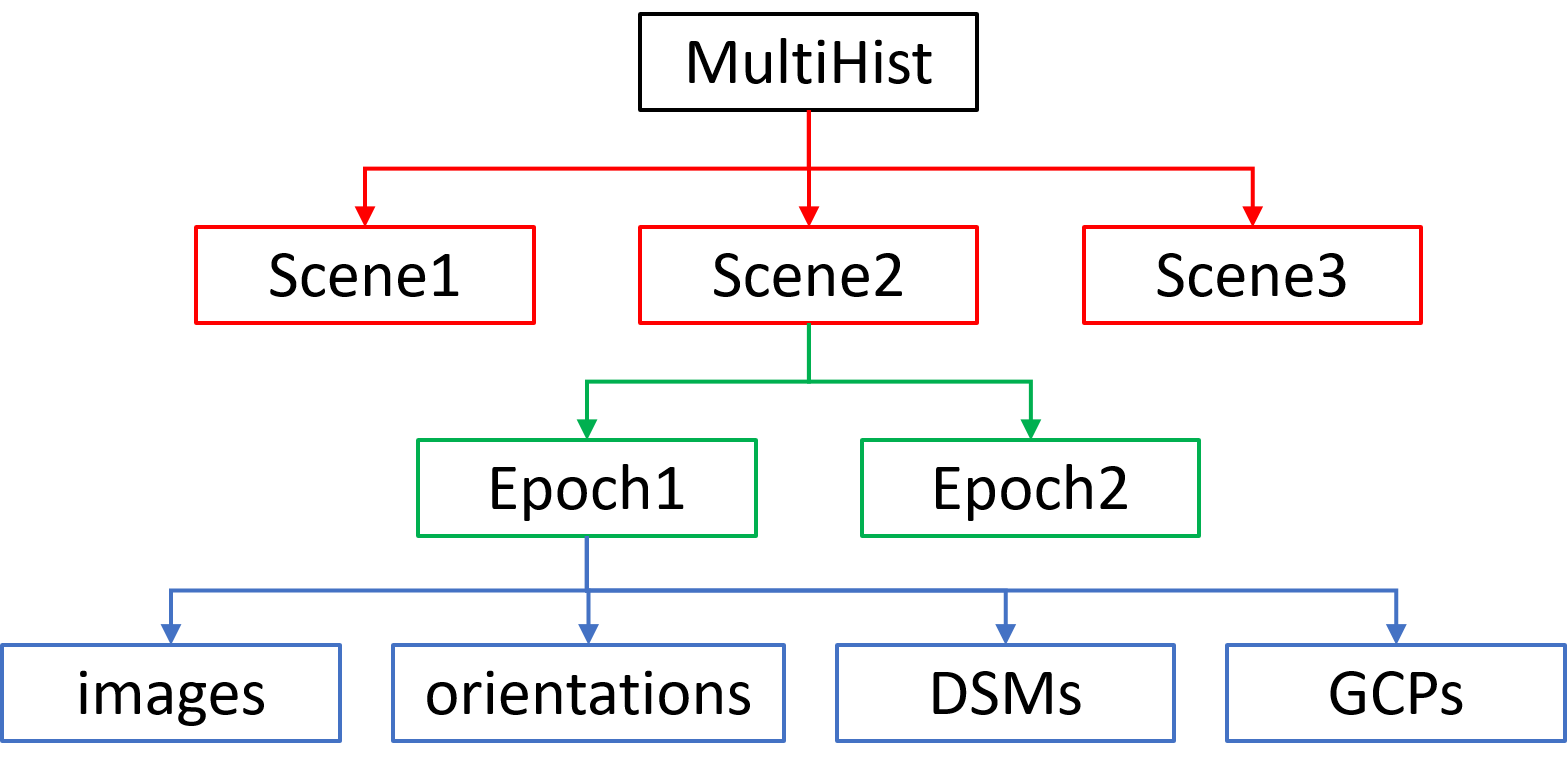
\includegraphics[width=7cm]{images/Chapitre5/MultiHist.png}
			\end{minipage}%
%		}
		\caption{Organization of our benchmark.}
		\label{multihist}
	\end{center}
\end{figure*}


\paragraph{Train a network with RGB images combined with \ac{DSM}s}
Another direction of our future work is to use both RGB images and \ac{DSM}s to train a neural network architecture in extracting robust features over time. 
As training data made from historical images is limited, it might be better to fine-tune existing models (e.g., SuperGlue). 
In order to validate if it improves matching performance to use RGB images and \ac{DSM}s at the same time, we did a comparison of using off-the-shelf SuperGlue model to match (1) RGB images only, (2) corresponding full resolution \ac{DSM}s only and (3) RGB images combined with \ac{DSM}s by concatenating keypoints. We choose a pair of roughly aligned images and feed them directly into SuperGlue without applying any \textit{tiling scheme} to keep the performance independent from irrelevant factors. The results are displayed in Figure \ref{RGBDSM}(c), (d) and (e) respectively, with their accuracy compared in Figure \ref{RGBDSM}(f). 
%As can be seen, Figure \ref{RGBDSM}(e) provides the most matches with best accuracy. 
As can be seen, it provides more matches with better accuracy when simply feeding concatenated keypoints to the ready-made model, it is reasonable to expect better performance after we fine-tune the model. 
%\ac{DSM}s.


\begin{figure*}[htbp]
	\begin{center}
		\subfigure[RGB image pair]{
			\begin{minipage}[t]{0.48\linewidth}
				\centering
				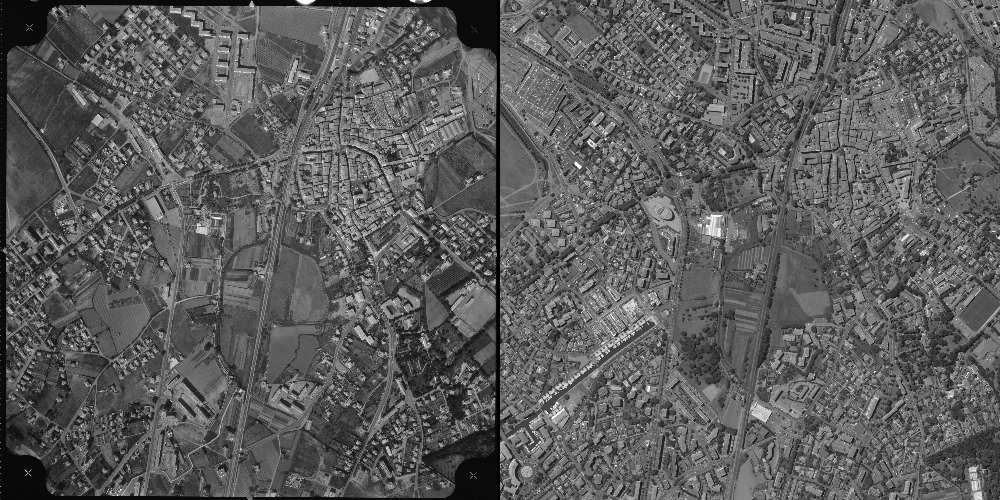
\includegraphics[width=6.5cm]{images/Chapitre5/RGB.png}
			\end{minipage}%
		}
		\subfigure[\ac{DSM} pair]{
			\begin{minipage}[t]{0.48\linewidth}
				\centering
				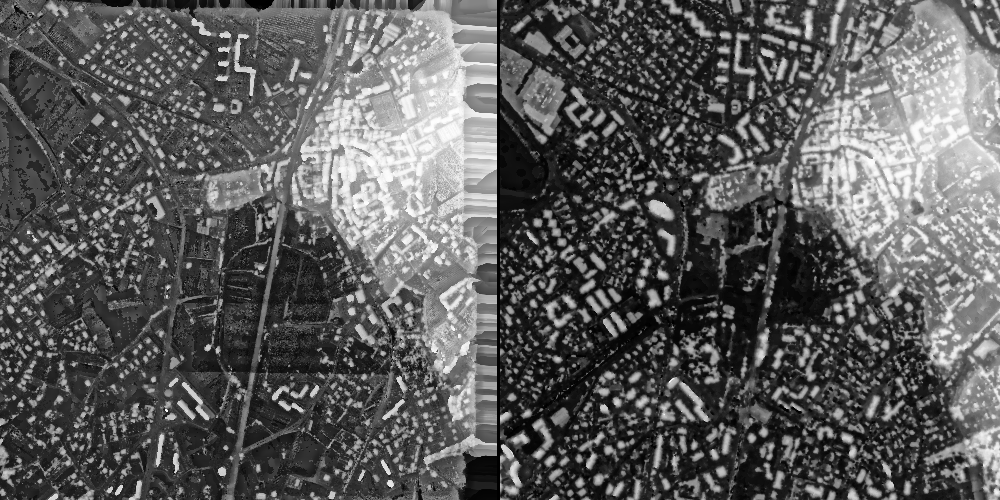
\includegraphics[width=6.5cm]{images/Chapitre5/DSM.png}
			\end{minipage}%
		}
		\subfigure[Matches on RGB images]{
			\begin{minipage}[t]{0.48\linewidth}
				\centering
				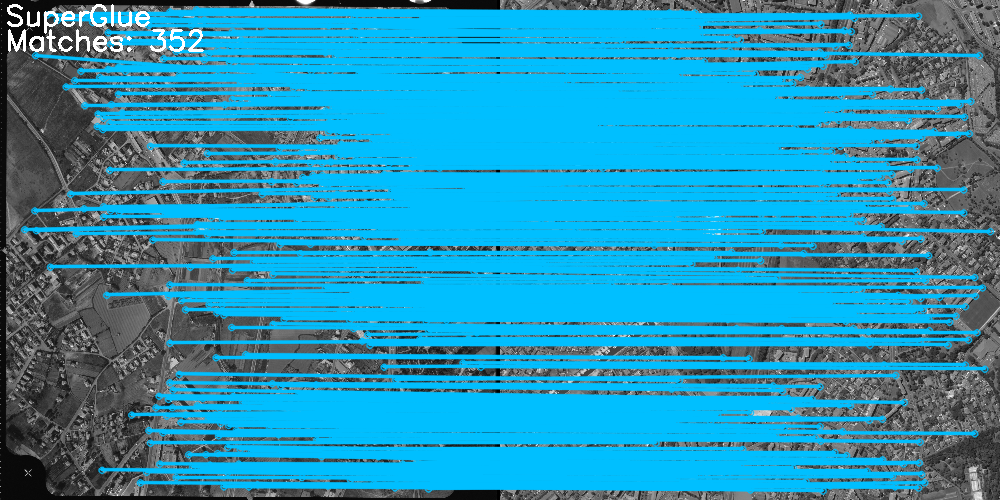
\includegraphics[width=6.5cm]{images/Chapitre5/RGBRes.png}
			\end{minipage}%
		}
		\subfigure[Matches on \ac{DSM}s]{
			\begin{minipage}[t]{0.48\linewidth}
				\centering
				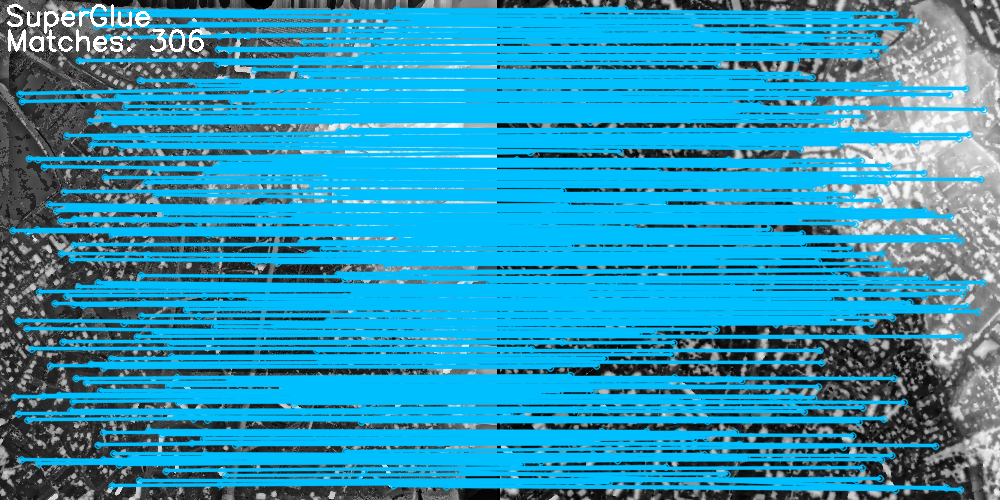
\includegraphics[width=6.5cm]{images/Chapitre5/DSMRes.png}
			\end{minipage}%
		}
		\subfigure[Matches on concatenation]{
			\begin{minipage}[t]{0.48\linewidth}
				\centering
				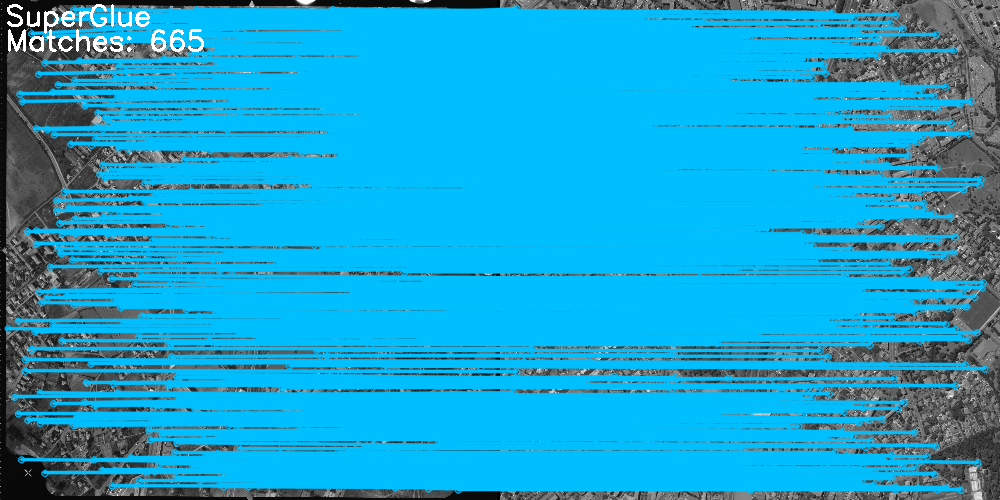
\includegraphics[width=6.5cm]{images/Chapitre5/CatRes.png}
			\end{minipage}%
		}
		\subfigure[Accuracy of (c-e)]{
			\begin{minipage}[t]{0.48\linewidth}
				\centering
				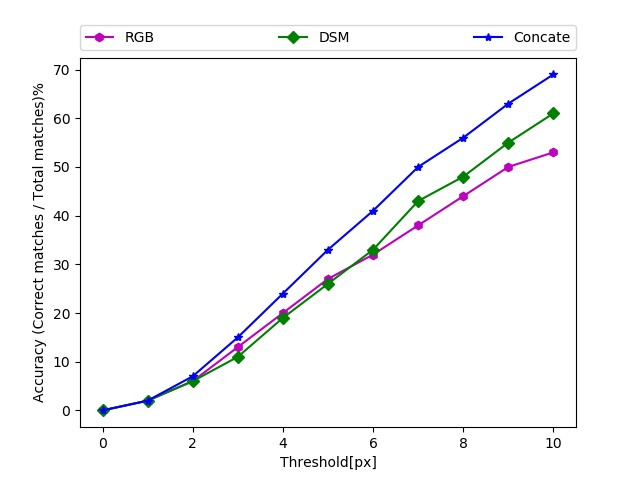
\includegraphics[width=5cm]{images/Chapitre5/TiePtAccuracy.jpg}
			\end{minipage}%
		}
		\caption{Comparison of SuperGlue applied on RGB images (c), \ac{DSM}s (d) and combined input by concatenating the keypoints (e). }
		\label{RGBDSM}
	\end{center}
\end{figure*} 

%The first attempt could be made with the simplest design as a starter: 
%论文的目标是什么,自己是怎么完成的,哪些子课题被研究了
%conclusion, 2 pages
%perspective, 1 page